\documentclass[paperwidth=90cm,paperheight=120cm,portrait]{baposter}
\usepackage[utf8]{inputenc}
\usepackage{cmap}
\usepackage[T1]{fontenc}
\usepackage[english]{babel}
% \usepackage{beamerposter}
% \usepackage[paperwidth=90cm,paperheight=100cm]{geometry}
% \geometry{paperwidth=90cm,paperheight=100cm}
\usepackage{biblatex}
\addbibresource{references.bib}

\usepackage{url}
\usepackage{breakurl}
% \usepackage{hyperref}

\usepackage{amsmath}
\usepackage{amsfonts}
\usepackage{amssymb}
\usepackage{amsthm}

\usepackage{graphicx}
\usepackage{tikz}
\usepackage{pgfplots}



%%%%%%%%%%%%%%%%%%%%%%%%%%%%%% Pacotes: tabelas %%%%%%%%%%%%%%%%%%%%%%%%%%%%%%
% \usepackage{multicol}
% \usepackage{multirow}

%%%%%%%%%%%%%%%%%%%%%%%%%%%%% Pacotes: algoritmos %%%%%%%%%%%%%%%%%%%%%%%%%%%%%
% \usepackage{algorithmic}
% \usepackage{algorithm}
% \floatname{algorithm}{Algoritmo}
% \renewcommand{\listalgorithmname}{Lista de Algoritmos}


%%%%%%%%%%%%%%%%%%%%%%%%%%%%%% Pacotes: códigos %%%%%%%%%%%%%%%%%%%%%%%%%%%%%%
\usepackage{textcomp}
\usepackage{listings}
\renewcommand\lstlistingname{Código}
\renewcommand\lstlistlistingname{Lista de Códigos}


%%%%%%%%%%%%%%%%%%%%%%%%%%%%%%% Pacotes: index %%%%%%%%%%%%%%%%%%%%%%%%%%%%%%%
% \usepackage{makeidx}
% \makeindex


%%%%%%%%%%%%%%%%%%%%%%%%%%%%%%% Pacotes: fontes %%%%%%%%%%%%%%%%%%%%%%%%%%%%%%
\usepackage{lmodern}
\usepackage{mathrsfs}


%%%%%%%%%%%%%%%%%%%%%%%%%%%%%%% Pacotes: LRS %%%%%%%%%%%%%%%%%%%%%%%%%%%%%%

%For Multicols
\usepackage{multicol}
% For Smaller
\usepackage{relsize} 



%%%%%%%%%%%%%%%%%%%%%%%%%%%%%%% Início do poster %%%%%%%%%%%%%%%%%%%%%%%%%%%%%%%
% \usetheme{Copenhagen}
% \setbeamertemplate{headline}{}
% \setbeamertemplate{footline}{}
\begin{document}


\begin{poster}{
 % Show grid to help with alignment
 grid=false,
 % Column spacing
 % colspacing=0.7em,
 % Color style
 headerColorOne=cyan!20!white!90!black,
 borderColor=cyan!30!white!90!black,
% Eye Catcher
 % eyecatcher=false,
 % Format of textbox
 % textborder=faded,
 % Format of text header
 headerborder=open,
 headershape=roundedright,
 headershade=plain,
 background=none,
 bgColorOne=cyan!10!white,
 headerheight=0.12\textheight}
 % Eye Catcher
 % NO EYECATCHER
 {
      % \includegraphics[width=0.08\linewidth]{track_frame_00010_06}
      % \includegraphics[width=0.08\linewidth]{track_frame_00450_06}
      % \includegraphics[width=0.08\linewidth]{track_frame_04999_06}
 }
 % Title
 {\sc\Huge perprof-py -- A Python Package for Performance Profile}
 % Authors
 { Raniere Gaia Costa da Silva, Abel Soares Siqueira, and Luiz Rafael dos Santos \\[1mm]
 \smaller \texttt{raniere@ime.unicamp.br, abel.s.siqueira@gmail.com, lrsantos11@gmail.com} }
 % University logo
 {
  % \begin{tabular}{r}
  %   \includegraphics[height=0.12\textheight]{logo}\\
  %   \raisebox{0em}[0em][0em]{\includegraphics[height=0.03\textheight]{msrlogo}}
  % \end{tabular}
 }

      
%%%%%%%%%%%%%%%%%%%%%%%%%%%%%%% Corpo do poster %%%%%%%%%%%%%%%%%%%%%%%%%%%%%%%
      \begin{posterbox}[name=intro,column=0,row=0,span=1]{Introduction}
        Benchmarking optimization packages are very important in optimization
        field, not only because it is one of the way to compare packages, but also
        to uncover deficiencies that could be overlooked. During benchmarking, one
        can obtain several informations, like CPU time, number of functions
        evaluations, number of iterations and so on. These informations, if
        presented as tables, can be difficult to be analyzed, due, for instance,
        to large amount of data. Therefore, researchers started testing tools to
        better process and understand this data.  One of the most widespread ways
        to do so is using Performance Profile graphics proposed by
        \textcite{Dolan2001}.
       \end{posterbox}

       \begin{posterbox}[name=perprof,below=intro]{Performance Profile}  

        The performance profile for a solver is the cumulative distribution
        function for a performance metric, e.g, CPU time, number of functions
        evaluations, number of iterations and so on.

        Given a set $P$ of problems and a set $S$ of solvers. For each problem $p
        \in P$ and solver $s \in S$, we define $t_{ps}$ as the computing time
        required to solve problem $p$ by solver $s$ and
        \begin{align*}
          r_{ps} = \frac{t_{ps}}{\min\{t_{ps}: s \in S\}}
        \end{align*}
        as the performance ratio of solver $s$ for the problem $p$ when compared
        with the best performance by any solver on this problem.

        \citeauthor{Dolan2001} define
        \begin{align*}
          \rho_s(\tau) = \frac{| \{p \in P: r_{ps} \leq \tau\} |}{| P |}
        \end{align*}
        where $\rho_s(\tau)$ is the probability for solver $s \in S$ to solve one
        problem within a factor $\tau \in \mathbb{R}$ of the best performance
        ratio. For a given $\tau$, the best solver is the one with the higher
        value for $\rho_s(\tau)$.

        One of the advantages of using performance profiles is the easily graphic
        analyse, it be relatively insensitive to changes in results on a small
        number of problems and also largely unaffected by small changes in
        results over many problems.
        \end{posterbox}

       \begin{posterbox}[name=perprof-py,below=perprof] {perprof-py}
       We implemented a free software that makes Performance
        Profile using data provided by user in a friendly manner. This software
        produces graphics in PDF using LaTeX with PGF/TikZ\nocite{TikZ} and
        pgfplots\nocite{pgfplots} packages, in PNG using
        matplotlib\nocite{Hunter:2007} and can also be easily extended to use with
        other plot library. The software is implemented in Python3 with support
        for internationalization and is available on
        \url{https://github.com/abelsiqueira/perprof-py}.
      \end{posterbox}

    \begin{posterbox}[name=features,below=perprof-py]{Features}
        Some of perprof-py features are:
        \begin{itemize}
          \item output LaTeX code,
          \item output bitmap (using matplotlib),
          \item options to treat some problems (e.g. spend time equals to
            zero),
          \item native internationalization support.

          \item Can be used in external tools that support Python
        \end{itemize}

    \end{posterbox}

 \begin{posterbox}[name=inputfile,column=1,span=2]{Input File}  
    %   \begin{block}{Input file}
        For every solver to be included in the benchmark there must be a file like
        the sample below:

        \begin{lstlisting}
        # Solver name
        Problem01 exit01 time01 objective01 primal01 dual01
        Problem02 exit02 time02 objective02 primal02 dual02
        Problem03 exit03 time03 objective03 primal03 dual03
        \end{lstlisting}

        Each file has 6 columns that means, in order:
        \begin{multicols}{2} 
          
        \begin{enumerate}
          \item The name of the problem;
          \item Exit flag;
          \item Time spent;
          \item Objective function value;
          \item Primal infeasibility;
          \item Dual infeasibility.
        \end{enumerate}
        \end{multicols} 
      % \end{block}
    % \end{column}
   \end{posterbox}
       \begin{posterbox}[name=output,column=1,span=2,below=inputfile]{Output Example}
        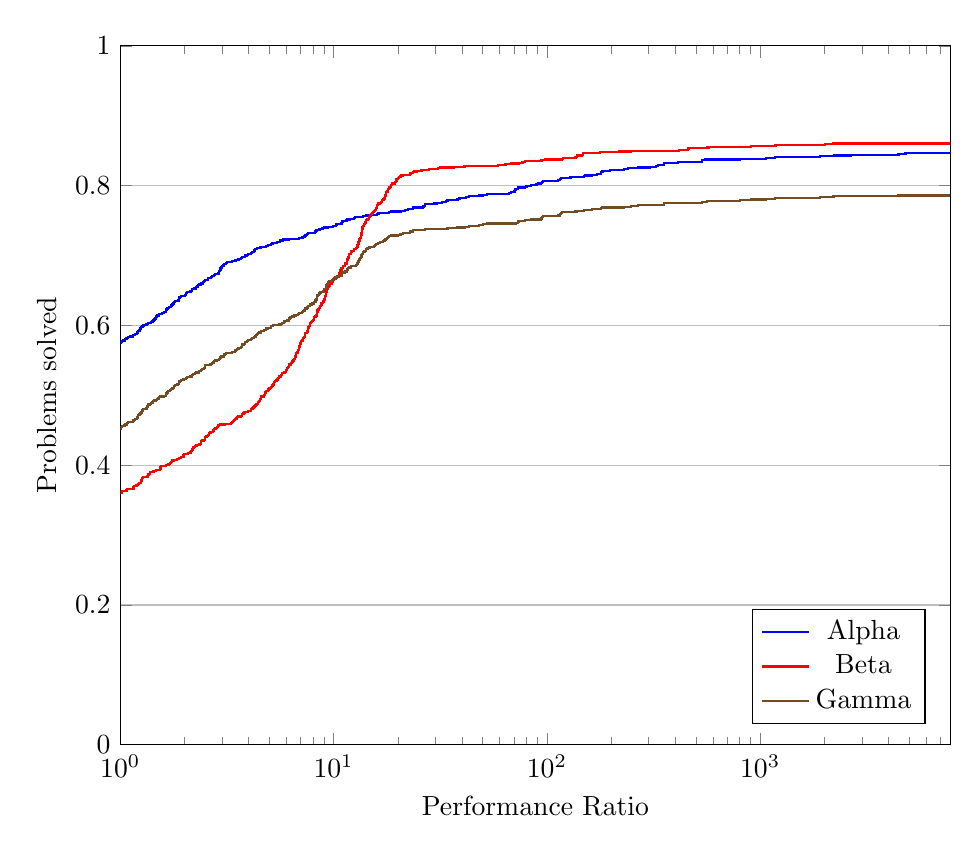
\begin{tikzpicture}
  \begin{semilogxaxis}[const plot, 
    xmin=1, xmax=7800.96,    ymin=0, ymax=1,
    ymajorgrids,
    ytick={0,0.2,0.4,0.6,0.8,1.0},
    xlabel={Performance Ratio}, ylabel={Problems solved},
    legend pos= south east,
    width=\textwidth
    ]
  \addplot+[mark=none, thick] coordinates {
    (1.0000,0.5750)
    (1.0070,0.5750)
    (1.0084,0.5762)
    (1.0144,0.5773)
    (1.0174,0.5773)
    (1.0195,0.5773)
    (1.0299,0.5785)
    (1.0476,0.5796)
    (1.0530,0.5808)
    (1.0690,0.5819)
    (1.0704,0.5819)
    (1.0713,0.5819)
    (1.0874,0.5830)
    (1.1086,0.5842)
    (1.1407,0.5853)
    (1.1446,0.5853)
    (1.1454,0.5865)
    (1.1539,0.5865)
    (1.1542,0.5865)
    (1.1595,0.5865)
    (1.1685,0.5876)
    (1.1920,0.5876)
    (1.1960,0.5888)
    (1.1964,0.5899)
    (1.2051,0.5911)
    (1.2130,0.5922)
    (1.2150,0.5922)
    (1.2157,0.5922)
    (1.2233,0.5922)
    (1.2310,0.5934)
    (1.2343,0.5945)
    (1.2419,0.5956)
    (1.2442,0.5968)
    (1.2477,0.5968)
    (1.2492,0.5968)
    (1.2528,0.5979)
    (1.2568,0.5979)
    (1.2614,0.5979)
    (1.2659,0.5979)
    (1.2688,0.5979)
    (1.2701,0.5991)
    (1.2741,0.5991)
    (1.2853,0.6002)
    (1.3258,0.6014)
    (1.3260,0.6025)
    (1.3342,0.6025)
    (1.3409,0.6025)
    (1.3453,0.6037)
    (1.3497,0.6037)
    (1.3577,0.6037)
    (1.3762,0.6037)
    (1.3822,0.6037)
    (1.3837,0.6037)
    (1.3944,0.6048)
    (1.4148,0.6060)
    (1.4219,0.6071)
    (1.4334,0.6071)
    (1.4455,0.6082)
    (1.4478,0.6094)
    (1.4614,0.6105)
    (1.4650,0.6105)
    (1.4713,0.6117)
    (1.4764,0.6128)
    (1.4828,0.6140)
    (1.5124,0.6151)
    (1.5234,0.6163)
    (1.5371,0.6163)
    (1.5448,0.6163)
    (1.5457,0.6163)
    (1.5459,0.6163)
    (1.5473,0.6163)
    (1.5648,0.6174)
    (1.6104,0.6186)
    (1.6191,0.6197)
    (1.6341,0.6208)
    (1.6386,0.6208)
    (1.6406,0.6220)
    (1.6492,0.6231)
    (1.6606,0.6243)
    (1.6758,0.6254)
    (1.6795,0.6254)
    (1.6824,0.6254)
    (1.6871,0.6266)
    (1.7179,0.6266)
    (1.7282,0.6266)
    (1.7351,0.6277)
    (1.7373,0.6289)
    (1.7470,0.6289)
    (1.7505,0.6300)
    (1.7538,0.6300)
    (1.7744,0.6312)
    (1.7809,0.6323)
    (1.7855,0.6334)
    (1.7871,0.6334)
    (1.8131,0.6346)
    (1.8482,0.6346)
    (1.8705,0.6357)
    (1.8866,0.6369)
    (1.8888,0.6380)
    (1.8903,0.6392)
    (1.8903,0.6392)
    (1.8959,0.6403)
    (1.9310,0.6415)
    (1.9338,0.6415)
    (1.9350,0.6426)
    (1.9738,0.6426)
    (1.9801,0.6426)
    (1.9805,0.6426)
    (1.9931,0.6426)
    (2.0049,0.6438)
    (2.0298,0.6449)
    (2.0364,0.6460)
    (2.0479,0.6472)
    (2.0557,0.6483)
    (2.0834,0.6483)
    (2.1300,0.6483)
    (2.1355,0.6495)
    (2.1447,0.6495)
    (2.1525,0.6495)
    (2.1675,0.6506)
    (2.1691,0.6518)
    (2.1728,0.6518)
    (2.1802,0.6518)
    (2.1891,0.6518)
    (2.1978,0.6518)
    (2.2057,0.6518)
    (2.2274,0.6529)
    (2.2334,0.6529)
    (2.2645,0.6541)
    (2.2682,0.6552)
    (2.2762,0.6552)
    (2.3033,0.6564)
    (2.3103,0.6575)
    (2.3346,0.6575)
    (2.3446,0.6586)
    (2.3537,0.6586)
    (2.3848,0.6586)
    (2.3884,0.6586)
    (2.3925,0.6598)
    (2.3965,0.6598)
    (2.4172,0.6598)
    (2.4290,0.6609)
    (2.4427,0.6621)
    (2.4635,0.6621)
    (2.4702,0.6632)
    (2.4877,0.6632)
    (2.4940,0.6632)
    (2.4963,0.6644)
    (2.5055,0.6644)
    (2.5334,0.6644)
    (2.5566,0.6644)
    (2.5576,0.6655)
    (2.5690,0.6655)
    (2.5711,0.6667)
    (2.5867,0.6678)
    (2.6128,0.6678)
    (2.6129,0.6678)
    (2.6244,0.6678)
    (2.6705,0.6678)
    (2.6734,0.6690)
    (2.6843,0.6701)
    (2.7011,0.6712)
    (2.7150,0.6712)
    (2.7374,0.6712)
    (2.7407,0.6712)
    (2.7589,0.6724)
    (2.7711,0.6724)
    (2.7743,0.6735)
    (2.8082,0.6735)
    (2.8438,0.6735)
    (2.8693,0.6735)
    (2.8867,0.6735)
    (2.8887,0.6747)
    (2.8971,0.6758)
    (2.9045,0.6770)
    (2.9067,0.6781)
    (2.9258,0.6793)
    (2.9314,0.6793)
    (2.9502,0.6804)
    (2.9511,0.6816)
    (2.9583,0.6827)
    (2.9856,0.6838)
    (2.9890,0.6850)
    (3.0469,0.6861)
    (3.0538,0.6873)
    (3.0777,0.6873)
    (3.1234,0.6884)
    (3.1389,0.6896)
    (3.1776,0.6907)
    (3.3158,0.6907)
    (3.3285,0.6907)
    (3.3310,0.6919)
    (3.3889,0.6919)
    (3.4172,0.6919)
    (3.4262,0.6919)
    (3.4459,0.6919)
    (3.4706,0.6930)
    (3.5070,0.6930)
    (3.5181,0.6930)
    (3.5597,0.6930)
    (3.5855,0.6942)
    (3.6172,0.6953)
    (3.6721,0.6953)
    (3.6884,0.6964)
    (3.7065,0.6964)
    (3.7335,0.6976)
    (3.7363,0.6976)
    (3.7834,0.6976)
    (3.8158,0.6976)
    (3.8332,0.6976)
    (3.8443,0.6987)
    (3.8518,0.6999)
    (3.9165,0.7010)
    (3.9576,0.7010)
    (3.9734,0.7022)
    (4.0932,0.7022)
    (4.1080,0.7033)
    (4.1185,0.7033)
    (4.1344,0.7045)
    (4.1610,0.7045)
    (4.2059,0.7045)
    (4.2169,0.7045)
    (4.2367,0.7056)
    (4.2442,0.7068)
    (4.2564,0.7068)
    (4.2636,0.7079)
    (4.2739,0.7090)
    (4.3089,0.7090)
    (4.3134,0.7090)
    (4.3684,0.7102)
    (4.3773,0.7102)
    (4.4109,0.7102)
    (4.4179,0.7102)
    (4.4840,0.7102)
    (4.5119,0.7102)
    (4.5324,0.7102)
    (4.5382,0.7102)
    (4.5483,0.7113)
    (4.5511,0.7113)
    (4.5561,0.7113)
    (4.5621,0.7113)
    (4.5835,0.7125)
    (4.7127,0.7125)
    (4.7244,0.7125)
    (4.7544,0.7125)
    (4.7717,0.7125)
    (4.7913,0.7125)
    (4.8051,0.7136)
    (4.8122,0.7136)
    (4.8133,0.7136)
    (4.9194,0.7136)
    (4.9229,0.7148)
    (4.9596,0.7148)
    (4.9755,0.7148)
    (5.0115,0.7148)
    (5.1018,0.7159)
    (5.1050,0.7159)
    (5.1238,0.7159)
    (5.1420,0.7171)
    (5.1743,0.7171)
    (5.1955,0.7182)
    (5.2207,0.7182)
    (5.2363,0.7182)
    (5.2376,0.7182)
    (5.2572,0.7182)
    (5.3329,0.7182)
    (5.4050,0.7182)
    (5.4227,0.7194)
    (5.4528,0.7194)
    (5.4599,0.7194)
    (5.4871,0.7194)
    (5.5686,0.7194)
    (5.5820,0.7194)
    (5.5943,0.7205)
    (5.6170,0.7216)
    (5.6466,0.7216)
    (5.6809,0.7216)
    (5.7205,0.7216)
    (5.7488,0.7216)
    (5.8096,0.7228)
    (5.8563,0.7228)
    (5.8876,0.7228)
    (5.9680,0.7228)
    (5.9987,0.7228)
    (6.0246,0.7228)
    (6.0437,0.7228)
    (6.0506,0.7228)
    (6.1231,0.7228)
    (6.1602,0.7239)
    (6.1826,0.7239)
    (6.1863,0.7239)
    (6.2083,0.7239)
    (6.2789,0.7239)
    (6.3053,0.7239)
    (6.4113,0.7239)
    (6.4133,0.7239)
    (6.4350,0.7239)
    (6.5088,0.7239)
    (6.5393,0.7239)
    (6.5700,0.7239)
    (6.5845,0.7239)
    (6.6010,0.7239)
    (6.6619,0.7239)
    (6.6724,0.7239)
    (6.6895,0.7239)
    (6.6938,0.7239)
    (6.7476,0.7239)
    (6.8067,0.7239)
    (6.8200,0.7239)
    (6.8300,0.7239)
    (6.8692,0.7239)
    (6.8768,0.7251)
    (6.8872,0.7251)
    (6.8895,0.7251)
    (6.9008,0.7251)
    (6.9304,0.7251)
    (6.9327,0.7251)
    (6.9696,0.7251)
    (6.9882,0.7251)
    (6.9952,0.7251)
    (7.0327,0.7251)
    (7.0611,0.7251)
    (7.1283,0.7251)
    (7.1472,0.7262)
    (7.1722,0.7262)
    (7.1747,0.7262)
    (7.1870,0.7262)
    (7.2466,0.7262)
    (7.3092,0.7274)
    (7.3430,0.7274)
    (7.3507,0.7274)
    (7.3546,0.7274)
    (7.3765,0.7274)
    (7.3940,0.7285)
    (7.4354,0.7297)
    (7.5066,0.7308)
    (7.5275,0.7308)
    (7.5356,0.7308)
    (7.5546,0.7308)
    (7.5655,0.7308)
    (7.5892,0.7320)
    (7.5984,0.7320)
    (7.6066,0.7320)
    (7.6177,0.7320)
    (7.6229,0.7320)
    (7.6791,0.7320)
    (7.7300,0.7320)
    (7.7357,0.7320)
    (7.7386,0.7320)
    (7.7414,0.7320)
    (7.8310,0.7320)
    (7.9588,0.7320)
    (8.0030,0.7320)
    (8.0361,0.7320)
    (8.0629,0.7320)
    (8.0733,0.7320)
    (8.0846,0.7320)
    (8.1497,0.7331)
    (8.2228,0.7342)
    (8.2306,0.7342)
    (8.2468,0.7342)
    (8.2825,0.7354)
    (8.3090,0.7365)
    (8.3419,0.7365)
    (8.3618,0.7365)
    (8.3719,0.7365)
    (8.3853,0.7365)
    (8.4020,0.7365)
    (8.4054,0.7365)
    (8.4088,0.7365)
    (8.5043,0.7365)
    (8.5112,0.7365)
    (8.5668,0.7365)
    (8.5933,0.7377)
    (8.6481,0.7377)
    (8.6695,0.7377)
    (8.7055,0.7377)
    (8.7454,0.7377)
    (8.7820,0.7377)
    (8.8737,0.7388)
    (8.9355,0.7388)
    (8.9660,0.7388)
    (9.0165,0.7400)
    (9.0433,0.7400)
    (9.0511,0.7400)
    (9.0943,0.7400)
    (9.1180,0.7400)
    (9.1459,0.7400)
    (9.1699,0.7400)
    (9.2061,0.7400)
    (9.2304,0.7400)
    (9.2386,0.7400)
    (9.2426,0.7400)
    (9.2590,0.7400)
    (9.2835,0.7400)
    (9.3248,0.7400)
    (9.3319,0.7400)
    (9.4001,0.7400)
    (9.4225,0.7411)
    (9.4424,0.7411)
    (9.5282,0.7411)
    (9.5979,0.7411)
    (9.6200,0.7411)
    (9.6554,0.7411)
    (9.8044,0.7411)
    (9.8135,0.7411)
    (9.9062,0.7411)
    (9.9065,0.7423)
    (9.9368,0.7423)
    (9.9722,0.7423)
    (9.9912,0.7423)
    (10.0390,0.7423)
    (10.2200,0.7423)
    (10.2344,0.7434)
    (10.3221,0.7446)
    (10.3820,0.7446)
    (10.4099,0.7446)
    (10.5597,0.7446)
    (10.6185,0.7446)
    (10.6563,0.7446)
    (10.7052,0.7446)
    (10.7320,0.7446)
    (10.7381,0.7446)
    (10.8243,0.7457)
    (10.8886,0.7457)
    (10.9000,0.7457)
    (10.9150,0.7468)
    (10.9155,0.7480)
    (11.0040,0.7491)
    (11.0785,0.7491)
    (11.0902,0.7491)
    (11.2932,0.7491)
    (11.2993,0.7491)
    (11.3237,0.7491)
    (11.5029,0.7503)
    (11.5102,0.7503)
    (11.5609,0.7503)
    (11.5732,0.7514)
    (11.5865,0.7514)
    (11.5993,0.7514)
    (11.6250,0.7514)
    (11.7094,0.7514)
    (11.7553,0.7514)
    (11.8483,0.7514)
    (11.8550,0.7514)
    (11.9292,0.7526)
    (12.0457,0.7526)
    (12.0526,0.7526)
    (12.1152,0.7526)
    (12.1715,0.7526)
    (12.4386,0.7526)
    (12.5128,0.7526)
    (12.5160,0.7537)
    (12.6143,0.7549)
    (12.7719,0.7549)
    (12.8345,0.7549)
    (12.8502,0.7549)
    (12.9374,0.7549)
    (12.9694,0.7549)
    (13.0177,0.7549)
    (13.0908,0.7549)
    (13.1731,0.7549)
    (13.2146,0.7549)
    (13.2313,0.7549)
    (13.2815,0.7549)
    (13.3322,0.7549)
    (13.4089,0.7549)
    (13.4347,0.7549)
    (13.4779,0.7549)
    (13.5126,0.7549)
    (13.5300,0.7549)
    (13.5388,0.7549)
    (13.5914,0.7549)
    (13.6002,0.7549)
    (13.6267,0.7549)
    (13.6711,0.7549)
    (13.6800,0.7549)
    (13.7219,0.7560)
    (13.7518,0.7560)
    (13.7971,0.7560)
    (13.8884,0.7560)
    (14.0184,0.7560)
    (14.0748,0.7560)
    (14.1222,0.7560)
    (14.1604,0.7560)
    (14.2152,0.7572)
    (14.2470,0.7572)
    (14.4333,0.7572)
    (14.5433,0.7572)
    (14.6041,0.7572)
    (14.6962,0.7572)
    (14.7687,0.7572)
    (14.8419,0.7572)
    (14.9157,0.7572)
    (14.9690,0.7572)
    (14.9723,0.7583)
    (15.1419,0.7583)
    (15.2742,0.7583)
    (15.4430,0.7583)
    (15.4657,0.7583)
    (15.6973,0.7583)
    (15.7918,0.7583)
    (15.8635,0.7583)
    (15.9358,0.7583)
    (15.9479,0.7583)
    (15.9601,0.7583)
    (16.0166,0.7595)
    (16.0210,0.7595)
    (16.1072,0.7595)
    (16.1692,0.7595)
    (16.2456,0.7606)
    (16.5782,0.7606)
    (16.6838,0.7606)
    (16.8446,0.7606)
    (16.9398,0.7606)
    (16.9810,0.7606)
    (17.2180,0.7606)
    (17.3175,0.7606)
    (17.3605,0.7606)
    (17.4327,0.7606)
    (17.4908,0.7606)
    (17.5683,0.7606)
    (17.5936,0.7606)
    (17.6083,0.7606)
    (17.6379,0.7606)
    (17.8481,0.7606)
    (17.8938,0.7606)
    (18.0013,0.7606)
    (18.0091,0.7606)
    (18.1414,0.7606)
    (18.2202,0.7606)
    (18.2696,0.7617)
    (18.3639,0.7617)
    (18.5858,0.7629)
    (18.5918,0.7629)
    (18.6245,0.7629)
    (18.8593,0.7629)
    (18.8763,0.7629)
    (19.4181,0.7629)
    (19.4541,0.7629)
    (19.6363,0.7629)
    (19.7286,0.7629)
    (19.7472,0.7629)
    (19.9160,0.7629)
    (20.0913,0.7629)
    (20.3218,0.7629)
    (20.5956,0.7629)
    (20.6311,0.7629)
    (20.7275,0.7640)
    (21.1055,0.7640)
    (21.5642,0.7652)
    (22.2494,0.7663)
    (22.7982,0.7663)
    (22.9594,0.7663)
    (23.5499,0.7675)
    (23.5738,0.7686)
    (23.6376,0.7686)
    (23.8792,0.7686)
    (24.5138,0.7686)
    (25.8350,0.7686)
    (26.3648,0.7698)
    (26.4208,0.7709)
    (26.7268,0.7721)
    (26.7664,0.7732)
    (28.1308,0.7732)
    (29.4922,0.7743)
    (30.5920,0.7755)
    (30.7839,0.7755)
    (31.5353,0.7755)
    (32.3252,0.7766)
    (33.7634,0.7778)
    (34.2434,0.7789)
    (36.4687,0.7789)
    (37.9353,0.7801)
    (38.1246,0.7812)
    (38.9201,0.7824)
    (41.0602,0.7824)
    (41.6904,0.7835)
    (43.1244,0.7847)
    (48.1244,0.7858)
    (50.3221,0.7869)
    (52.5491,0.7881)
    (59.1555,0.7881)
    (63.9696,0.7881)
    (66.2847,0.7892)
    (67.6969,0.7892)
    (68.1393,0.7904)
    (70.0878,0.7915)
    (70.6808,0.7927)
    (71.0216,0.7938)
    (71.2535,0.7950)
    (72.9546,0.7961)
    (73.6136,0.7973)
    (74.0758,0.7973)
    (76.8188,0.7973)
    (78.5092,0.7984)
    (78.9366,0.7984)
    (80.2296,0.7995)
    (84.1233,0.8007)
    (89.3195,0.8018)
    (91.1035,0.8030)
    (93.9500,0.8041)
    (94.4164,0.8041)
    (94.8362,0.8053)
    (95.7332,0.8064)
    (98.4011,0.8064)
    (112.9562,0.8076)
    (114.9805,0.8087)
    (115.2740,0.8099)
    (116.1100,0.8110)
    (117.9449,0.8110)
    (118.9275,0.8110)
    (129.1242,0.8121)
    (136.0885,0.8121)
    (138.2389,0.8121)
    (138.6691,0.8121)
    (145.1715,0.8121)
    (147.6357,0.8121)
    (147.8139,0.8121)
    (148.7564,0.8133)
    (150.4310,0.8144)
    (163.2343,0.8156)
    (172.3965,0.8167)
    (178.1343,0.8167)
    (179.9448,0.8179)
    (180.0328,0.8190)
    (180.8403,0.8202)
    (182.4376,0.8213)
    (197.2343,0.8225)
    (217.5449,0.8225)
    (229.9470,0.8236)
    (239.2197,0.8247)
    (247.6605,0.8247)
    (266.9545,0.8259)
    (303.3250,0.8270)
    (323.9000,0.8282)
    (331.9400,0.8293)
    (353.0045,0.8305)
    (353.9860,0.8316)
    (355.2810,0.8328)
    (412.7200,0.8339)
    (416.6573,0.8339)
    (457.1390,0.8339)
    (461.6179,0.8339)
    (532.4860,0.8351)
    (535.2500,0.8362)
    (549.8680,0.8373)
    (565.4773,0.8373)
    (572.7256,0.8373)
    (805.6160,0.8385)
    (906.8762,0.8385)
    (1062.5660,0.8396)
    (1176.1676,0.8408)
    (1179.2855,0.8408)
    (1906.5143,0.8419)
    (2014.4500,0.8419)
    (2206.6033,0.8419)
    (2224.1833,0.8431)
    (2671.1500,0.8442)
    (4452.6333,0.8454)
    (4798.7400,0.8465)
    (7800.9600,0.8477)
  };
  \addlegendentry{Alpha}
  \addplot+[mark=none, thick] coordinates {
    (1.0000,0.3597)
    (1.0070,0.3608)
    (1.0084,0.3608)
    (1.0144,0.3608)
    (1.0174,0.3620)
    (1.0195,0.3631)
    (1.0299,0.3631)
    (1.0476,0.3631)
    (1.0530,0.3631)
    (1.0690,0.3631)
    (1.0704,0.3643)
    (1.0713,0.3654)
    (1.0874,0.3654)
    (1.1086,0.3654)
    (1.1407,0.3654)
    (1.1446,0.3666)
    (1.1454,0.3666)
    (1.1539,0.3677)
    (1.1542,0.3688)
    (1.1595,0.3700)
    (1.1685,0.3700)
    (1.1920,0.3711)
    (1.1960,0.3711)
    (1.1964,0.3711)
    (1.2051,0.3711)
    (1.2130,0.3711)
    (1.2150,0.3723)
    (1.2157,0.3734)
    (1.2233,0.3746)
    (1.2310,0.3746)
    (1.2343,0.3746)
    (1.2419,0.3746)
    (1.2442,0.3746)
    (1.2477,0.3757)
    (1.2492,0.3769)
    (1.2528,0.3769)
    (1.2568,0.3780)
    (1.2614,0.3792)
    (1.2659,0.3803)
    (1.2688,0.3814)
    (1.2701,0.3814)
    (1.2741,0.3826)
    (1.2853,0.3826)
    (1.3258,0.3826)
    (1.3260,0.3826)
    (1.3342,0.3837)
    (1.3409,0.3849)
    (1.3453,0.3849)
    (1.3497,0.3860)
    (1.3577,0.3872)
    (1.3762,0.3883)
    (1.3822,0.3895)
    (1.3837,0.3906)
    (1.3944,0.3906)
    (1.4148,0.3906)
    (1.4219,0.3906)
    (1.4334,0.3918)
    (1.4455,0.3918)
    (1.4478,0.3918)
    (1.4614,0.3918)
    (1.4650,0.3929)
    (1.4713,0.3929)
    (1.4764,0.3929)
    (1.4828,0.3929)
    (1.5124,0.3929)
    (1.5234,0.3929)
    (1.5371,0.3940)
    (1.5448,0.3952)
    (1.5457,0.3963)
    (1.5459,0.3975)
    (1.5473,0.3986)
    (1.5648,0.3986)
    (1.6104,0.3986)
    (1.6191,0.3986)
    (1.6341,0.3986)
    (1.6386,0.3998)
    (1.6406,0.3998)
    (1.6492,0.3998)
    (1.6606,0.3998)
    (1.6758,0.3998)
    (1.6795,0.4009)
    (1.6824,0.4021)
    (1.6871,0.4021)
    (1.7179,0.4032)
    (1.7282,0.4044)
    (1.7351,0.4044)
    (1.7373,0.4044)
    (1.7470,0.4055)
    (1.7505,0.4055)
    (1.7538,0.4066)
    (1.7744,0.4066)
    (1.7809,0.4066)
    (1.7855,0.4066)
    (1.7871,0.4078)
    (1.8131,0.4078)
    (1.8482,0.4089)
    (1.8705,0.4089)
    (1.8866,0.4089)
    (1.8888,0.4089)
    (1.8903,0.4089)
    (1.8903,0.4101)
    (1.8959,0.4101)
    (1.9310,0.4101)
    (1.9338,0.4112)
    (1.9350,0.4112)
    (1.9738,0.4124)
    (1.9801,0.4135)
    (1.9805,0.4147)
    (1.9931,0.4158)
    (2.0049,0.4158)
    (2.0298,0.4158)
    (2.0364,0.4158)
    (2.0479,0.4158)
    (2.0557,0.4158)
    (2.0834,0.4170)
    (2.1300,0.4181)
    (2.1355,0.4181)
    (2.1447,0.4192)
    (2.1525,0.4204)
    (2.1675,0.4204)
    (2.1691,0.4204)
    (2.1728,0.4215)
    (2.1802,0.4227)
    (2.1891,0.4238)
    (2.1978,0.4250)
    (2.2057,0.4261)
    (2.2274,0.4261)
    (2.2334,0.4273)
    (2.2645,0.4273)
    (2.2682,0.4273)
    (2.2762,0.4284)
    (2.3033,0.4284)
    (2.3103,0.4284)
    (2.3346,0.4296)
    (2.3446,0.4296)
    (2.3537,0.4307)
    (2.3848,0.4318)
    (2.3884,0.4330)
    (2.3925,0.4330)
    (2.3965,0.4341)
    (2.4172,0.4353)
    (2.4290,0.4353)
    (2.4427,0.4353)
    (2.4635,0.4364)
    (2.4702,0.4364)
    (2.4877,0.4376)
    (2.4940,0.4387)
    (2.4963,0.4387)
    (2.5055,0.4399)
    (2.5334,0.4410)
    (2.5566,0.4422)
    (2.5576,0.4422)
    (2.5690,0.4433)
    (2.5711,0.4433)
    (2.5867,0.4433)
    (2.6128,0.4444)
    (2.6129,0.4456)
    (2.6244,0.4467)
    (2.6705,0.4479)
    (2.6734,0.4479)
    (2.6843,0.4479)
    (2.7011,0.4479)
    (2.7150,0.4490)
    (2.7374,0.4502)
    (2.7407,0.4513)
    (2.7589,0.4513)
    (2.7711,0.4525)
    (2.7743,0.4525)
    (2.8082,0.4536)
    (2.8438,0.4548)
    (2.8693,0.4559)
    (2.8867,0.4570)
    (2.8887,0.4570)
    (2.8971,0.4570)
    (2.9045,0.4570)
    (2.9067,0.4570)
    (2.9258,0.4570)
    (2.9314,0.4582)
    (2.9502,0.4582)
    (2.9511,0.4582)
    (2.9583,0.4582)
    (2.9856,0.4582)
    (2.9890,0.4582)
    (3.0469,0.4582)
    (3.0538,0.4582)
    (3.0777,0.4593)
    (3.1234,0.4593)
    (3.1389,0.4593)
    (3.1776,0.4593)
    (3.3158,0.4605)
    (3.3285,0.4616)
    (3.3310,0.4616)
    (3.3889,0.4628)
    (3.4172,0.4639)
    (3.4262,0.4651)
    (3.4459,0.4662)
    (3.4706,0.4662)
    (3.5070,0.4674)
    (3.5181,0.4685)
    (3.5597,0.4696)
    (3.5855,0.4696)
    (3.6172,0.4696)
    (3.6721,0.4708)
    (3.6884,0.4708)
    (3.7065,0.4719)
    (3.7335,0.4719)
    (3.7363,0.4731)
    (3.7834,0.4742)
    (3.8158,0.4754)
    (3.8332,0.4765)
    (3.8443,0.4765)
    (3.8518,0.4765)
    (3.9165,0.4765)
    (3.9576,0.4777)
    (3.9734,0.4777)
    (4.0932,0.4788)
    (4.1080,0.4788)
    (4.1185,0.4800)
    (4.1344,0.4800)
    (4.1610,0.4811)
    (4.2059,0.4822)
    (4.2169,0.4834)
    (4.2367,0.4834)
    (4.2442,0.4834)
    (4.2564,0.4845)
    (4.2636,0.4845)
    (4.2739,0.4845)
    (4.3089,0.4857)
    (4.3134,0.4868)
    (4.3684,0.4868)
    (4.3773,0.4880)
    (4.4109,0.4891)
    (4.4179,0.4903)
    (4.4840,0.4914)
    (4.5119,0.4926)
    (4.5324,0.4937)
    (4.5382,0.4948)
    (4.5483,0.4948)
    (4.5511,0.4960)
    (4.5561,0.4971)
    (4.5621,0.4983)
    (4.5835,0.4983)
    (4.7127,0.4994)
    (4.7244,0.5006)
    (4.7544,0.5017)
    (4.7717,0.5029)
    (4.7913,0.5040)
    (4.8051,0.5040)
    (4.8122,0.5052)
    (4.8133,0.5063)
    (4.9194,0.5074)
    (4.9229,0.5074)
    (4.9596,0.5086)
    (4.9755,0.5097)
    (5.0115,0.5109)
    (5.1018,0.5109)
    (5.1050,0.5120)
    (5.1238,0.5132)
    (5.1420,0.5132)
    (5.1743,0.5143)
    (5.1955,0.5143)
    (5.2207,0.5155)
    (5.2363,0.5166)
    (5.2376,0.5178)
    (5.2572,0.5189)
    (5.3329,0.5200)
    (5.4050,0.5212)
    (5.4227,0.5212)
    (5.4528,0.5223)
    (5.4599,0.5235)
    (5.4871,0.5246)
    (5.5686,0.5258)
    (5.5820,0.5269)
    (5.5943,0.5269)
    (5.6170,0.5269)
    (5.6466,0.5281)
    (5.6809,0.5292)
    (5.7205,0.5304)
    (5.7488,0.5315)
    (5.8096,0.5315)
    (5.8563,0.5326)
    (5.8876,0.5338)
    (5.9680,0.5349)
    (5.9987,0.5361)
    (6.0246,0.5372)
    (6.0437,0.5384)
    (6.0506,0.5395)
    (6.1231,0.5407)
    (6.1602,0.5407)
    (6.1826,0.5418)
    (6.1863,0.5430)
    (6.2083,0.5441)
    (6.2789,0.5452)
    (6.3053,0.5464)
    (6.4113,0.5475)
    (6.4133,0.5487)
    (6.4350,0.5498)
    (6.5088,0.5510)
    (6.5393,0.5521)
    (6.5700,0.5533)
    (6.5845,0.5544)
    (6.6010,0.5556)
    (6.6619,0.5567)
    (6.6724,0.5578)
    (6.6895,0.5590)
    (6.6938,0.5601)
    (6.7476,0.5613)
    (6.8067,0.5624)
    (6.8200,0.5636)
    (6.8300,0.5647)
    (6.8692,0.5659)
    (6.8768,0.5659)
    (6.8872,0.5670)
    (6.8895,0.5682)
    (6.9008,0.5693)
    (6.9304,0.5704)
    (6.9327,0.5716)
    (6.9696,0.5727)
    (6.9882,0.5739)
    (6.9952,0.5750)
    (7.0327,0.5762)
    (7.0611,0.5773)
    (7.1283,0.5785)
    (7.1472,0.5785)
    (7.1722,0.5796)
    (7.1747,0.5808)
    (7.1870,0.5819)
    (7.2466,0.5830)
    (7.3092,0.5830)
    (7.3430,0.5842)
    (7.3507,0.5865)
    (7.3546,0.5876)
    (7.3765,0.5888)
    (7.3940,0.5888)
    (7.4354,0.5888)
    (7.5066,0.5888)
    (7.5275,0.5899)
    (7.5356,0.5911)
    (7.5546,0.5922)
    (7.5655,0.5934)
    (7.5892,0.5934)
    (7.5984,0.5945)
    (7.6066,0.5956)
    (7.6177,0.5968)
    (7.6229,0.5979)
    (7.6791,0.5991)
    (7.7300,0.6002)
    (7.7357,0.6014)
    (7.7386,0.6025)
    (7.7414,0.6037)
    (7.8310,0.6048)
    (7.9588,0.6060)
    (8.0030,0.6071)
    (8.0361,0.6082)
    (8.0629,0.6094)
    (8.0733,0.6105)
    (8.0846,0.6117)
    (8.1497,0.6117)
    (8.2228,0.6117)
    (8.2306,0.6128)
    (8.2468,0.6140)
    (8.2825,0.6140)
    (8.3090,0.6140)
    (8.3419,0.6151)
    (8.3618,0.6163)
    (8.3719,0.6174)
    (8.3853,0.6186)
    (8.4020,0.6197)
    (8.4054,0.6208)
    (8.4088,0.6220)
    (8.5043,0.6231)
    (8.5112,0.6243)
    (8.5668,0.6254)
    (8.5933,0.6254)
    (8.6481,0.6266)
    (8.6695,0.6277)
    (8.7055,0.6289)
    (8.7454,0.6300)
    (8.7820,0.6323)
    (8.8737,0.6323)
    (8.9355,0.6334)
    (8.9660,0.6346)
    (9.0165,0.6346)
    (9.0433,0.6357)
    (9.0511,0.6369)
    (9.0943,0.6380)
    (9.1180,0.6392)
    (9.1459,0.6415)
    (9.1699,0.6426)
    (9.2061,0.6438)
    (9.2304,0.6449)
    (9.2386,0.6460)
    (9.2426,0.6483)
    (9.2590,0.6495)
    (9.2835,0.6506)
    (9.3248,0.6518)
    (9.3319,0.6529)
    (9.4001,0.6541)
    (9.4225,0.6541)
    (9.4424,0.6552)
    (9.5282,0.6564)
    (9.5979,0.6575)
    (9.6200,0.6586)
    (9.6554,0.6598)
    (9.8044,0.6609)
    (9.8135,0.6621)
    (9.9062,0.6632)
    (9.9065,0.6632)
    (9.9368,0.6644)
    (9.9722,0.6655)
    (9.9912,0.6667)
    (10.0390,0.6678)
    (10.2200,0.6690)
    (10.2344,0.6690)
    (10.3221,0.6690)
    (10.3820,0.6701)
    (10.4099,0.6712)
    (10.5597,0.6724)
    (10.6185,0.6735)
    (10.6563,0.6747)
    (10.7052,0.6770)
    (10.7320,0.6781)
    (10.7381,0.6793)
    (10.8243,0.6793)
    (10.8886,0.6804)
    (10.9000,0.6816)
    (10.9150,0.6816)
    (10.9155,0.6816)
    (11.0040,0.6816)
    (11.0785,0.6827)
    (11.0902,0.6850)
    (11.2932,0.6861)
    (11.2993,0.6873)
    (11.3237,0.6884)
    (11.5029,0.6884)
    (11.5102,0.6896)
    (11.5609,0.6907)
    (11.5732,0.6907)
    (11.5865,0.6919)
    (11.5993,0.6930)
    (11.6250,0.6942)
    (11.7094,0.6964)
    (11.7553,0.6976)
    (11.8483,0.6999)
    (11.8550,0.7022)
    (11.9292,0.7022)
    (12.0457,0.7033)
    (12.0526,0.7045)
    (12.1152,0.7056)
    (12.1715,0.7068)
    (12.4386,0.7079)
    (12.5128,0.7090)
    (12.5160,0.7090)
    (12.6143,0.7090)
    (12.7719,0.7102)
    (12.8345,0.7113)
    (12.8502,0.7125)
    (12.9374,0.7148)
    (12.9694,0.7159)
    (13.0177,0.7171)
    (13.0908,0.7194)
    (13.1731,0.7205)
    (13.2146,0.7216)
    (13.2313,0.7228)
    (13.2815,0.7239)
    (13.3322,0.7251)
    (13.4089,0.7262)
    (13.4347,0.7274)
    (13.4779,0.7297)
    (13.5126,0.7308)
    (13.5300,0.7320)
    (13.5388,0.7331)
    (13.5914,0.7354)
    (13.6002,0.7365)
    (13.6267,0.7377)
    (13.6711,0.7388)
    (13.6800,0.7400)
    (13.7219,0.7400)
    (13.7518,0.7411)
    (13.7971,0.7423)
    (13.8884,0.7446)
    (14.0184,0.7457)
    (14.0748,0.7468)
    (14.1222,0.7480)
    (14.1604,0.7491)
    (14.2152,0.7491)
    (14.2470,0.7503)
    (14.4333,0.7514)
    (14.5433,0.7526)
    (14.6041,0.7537)
    (14.6962,0.7549)
    (14.7687,0.7560)
    (14.8419,0.7572)
    (14.9157,0.7583)
    (14.9690,0.7595)
    (14.9723,0.7595)
    (15.1419,0.7606)
    (15.2742,0.7617)
    (15.4430,0.7629)
    (15.4657,0.7640)
    (15.6973,0.7652)
    (15.7918,0.7663)
    (15.8635,0.7675)
    (15.9358,0.7686)
    (15.9479,0.7698)
    (15.9601,0.7709)
    (16.0166,0.7709)
    (16.0210,0.7721)
    (16.1072,0.7732)
    (16.1692,0.7743)
    (16.2456,0.7743)
    (16.5782,0.7755)
    (16.6838,0.7766)
    (16.8446,0.7778)
    (16.9398,0.7789)
    (16.9810,0.7801)
    (17.2180,0.7812)
    (17.3175,0.7824)
    (17.3605,0.7835)
    (17.4327,0.7847)
    (17.4908,0.7858)
    (17.5683,0.7869)
    (17.5936,0.7881)
    (17.6083,0.7892)
    (17.6379,0.7904)
    (17.8481,0.7915)
    (17.8938,0.7927)
    (18.0013,0.7938)
    (18.0091,0.7950)
    (18.1414,0.7961)
    (18.2202,0.7973)
    (18.2696,0.7973)
    (18.3639,0.7984)
    (18.5858,0.7984)
    (18.5918,0.7995)
    (18.6245,0.8007)
    (18.8593,0.8018)
    (18.8763,0.8030)
    (19.4181,0.8041)
    (19.4541,0.8053)
    (19.6363,0.8064)
    (19.7286,0.8076)
    (19.7472,0.8087)
    (19.9160,0.8099)
    (20.0913,0.8110)
    (20.3218,0.8121)
    (20.5956,0.8133)
    (20.6311,0.8144)
    (20.7275,0.8144)
    (21.1055,0.8156)
    (21.5642,0.8156)
    (22.2494,0.8156)
    (22.7982,0.8167)
    (22.9594,0.8179)
    (23.5499,0.8179)
    (23.5738,0.8179)
    (23.6376,0.8190)
    (23.8792,0.8202)
    (24.5138,0.8213)
    (25.8350,0.8225)
    (26.3648,0.8225)
    (26.4208,0.8225)
    (26.7268,0.8225)
    (26.7664,0.8225)
    (28.1308,0.8236)
    (29.4922,0.8236)
    (30.5920,0.8236)
    (30.7839,0.8247)
    (31.5353,0.8259)
    (32.3252,0.8259)
    (33.7634,0.8259)
    (34.2434,0.8259)
    (36.4687,0.8270)
    (37.9353,0.8270)
    (38.1246,0.8270)
    (38.9201,0.8270)
    (41.0602,0.8282)
    (41.6904,0.8282)
    (43.1244,0.8282)
    (48.1244,0.8282)
    (50.3221,0.8282)
    (52.5491,0.8282)
    (59.1555,0.8293)
    (63.9696,0.8305)
    (66.2847,0.8305)
    (67.6969,0.8316)
    (68.1393,0.8316)
    (70.0878,0.8316)
    (70.6808,0.8316)
    (71.0216,0.8316)
    (71.2535,0.8316)
    (72.9546,0.8316)
    (73.6136,0.8316)
    (74.0758,0.8328)
    (76.8188,0.8339)
    (78.5092,0.8339)
    (78.9366,0.8351)
    (80.2296,0.8351)
    (84.1233,0.8351)
    (89.3195,0.8351)
    (91.1035,0.8351)
    (93.9500,0.8351)
    (94.4164,0.8362)
    (94.8362,0.8362)
    (95.7332,0.8362)
    (98.4011,0.8373)
    (112.9562,0.8373)
    (114.9805,0.8373)
    (115.2740,0.8373)
    (116.1100,0.8373)
    (117.9449,0.8385)
    (118.9275,0.8396)
    (129.1242,0.8396)
    (136.0885,0.8408)
    (138.2389,0.8419)
    (138.6691,0.8431)
    (145.1715,0.8442)
    (147.6357,0.8454)
    (147.8139,0.8465)
    (148.7564,0.8465)
    (150.4310,0.8465)
    (163.2343,0.8465)
    (172.3965,0.8465)
    (178.1343,0.8477)
    (179.9448,0.8477)
    (180.0328,0.8477)
    (180.8403,0.8477)
    (182.4376,0.8477)
    (197.2343,0.8477)
    (217.5449,0.8488)
    (229.9470,0.8488)
    (239.2197,0.8488)
    (247.6605,0.8499)
    (266.9545,0.8499)
    (303.3250,0.8499)
    (323.9000,0.8499)
    (331.9400,0.8499)
    (353.0045,0.8499)
    (353.9860,0.8499)
    (355.2810,0.8499)
    (412.7200,0.8499)
    (416.6573,0.8511)
    (457.1390,0.8522)
    (461.6179,0.8534)
    (532.4860,0.8534)
    (535.2500,0.8534)
    (549.8680,0.8534)
    (565.4773,0.8545)
    (572.7256,0.8557)
    (805.6160,0.8557)
    (906.8762,0.8568)
    (1062.5660,0.8568)
    (1176.1676,0.8568)
    (1179.2855,0.8580)
    (1906.5143,0.8580)
    (2014.4500,0.8591)
    (2206.6033,0.8603)
    (2224.1833,0.8603)
    (2671.1500,0.8603)
    (4452.6333,0.8603)
    (4798.7400,0.8603)
    (7800.9600,0.8603)
  };
  \addlegendentry{Beta}
  \addplot+[mark=none, thick] coordinates {
    (1.0000,0.4525)
    (1.0070,0.4536)
    (1.0084,0.4548)
    (1.0144,0.4548)
    (1.0174,0.4559)
    (1.0195,0.4559)
    (1.0299,0.4559)
    (1.0476,0.4570)
    (1.0530,0.4582)
    (1.0690,0.4593)
    (1.0704,0.4593)
    (1.0713,0.4605)
    (1.0874,0.4616)
    (1.1086,0.4616)
    (1.1407,0.4616)
    (1.1446,0.4628)
    (1.1454,0.4639)
    (1.1539,0.4651)
    (1.1542,0.4651)
    (1.1595,0.4651)
    (1.1685,0.4662)
    (1.1920,0.4662)
    (1.1960,0.4662)
    (1.1964,0.4674)
    (1.2051,0.4685)
    (1.2130,0.4696)
    (1.2150,0.4708)
    (1.2157,0.4719)
    (1.2233,0.4719)
    (1.2310,0.4731)
    (1.2343,0.4731)
    (1.2419,0.4731)
    (1.2442,0.4742)
    (1.2477,0.4742)
    (1.2492,0.4742)
    (1.2528,0.4754)
    (1.2568,0.4754)
    (1.2614,0.4765)
    (1.2659,0.4777)
    (1.2688,0.4777)
    (1.2701,0.4788)
    (1.2741,0.4800)
    (1.2853,0.4800)
    (1.3258,0.4811)
    (1.3260,0.4822)
    (1.3342,0.4834)
    (1.3409,0.4845)
    (1.3453,0.4857)
    (1.3497,0.4857)
    (1.3577,0.4868)
    (1.3762,0.4868)
    (1.3822,0.4880)
    (1.3837,0.4880)
    (1.3944,0.4891)
    (1.4148,0.4903)
    (1.4219,0.4914)
    (1.4334,0.4914)
    (1.4455,0.4926)
    (1.4478,0.4926)
    (1.4614,0.4926)
    (1.4650,0.4937)
    (1.4713,0.4937)
    (1.4764,0.4937)
    (1.4828,0.4948)
    (1.5124,0.4960)
    (1.5234,0.4971)
    (1.5371,0.4983)
    (1.5448,0.4983)
    (1.5457,0.4983)
    (1.5459,0.4983)
    (1.5473,0.4983)
    (1.5648,0.4983)
    (1.6104,0.4994)
    (1.6191,0.4994)
    (1.6341,0.5006)
    (1.6386,0.5017)
    (1.6406,0.5017)
    (1.6492,0.5029)
    (1.6606,0.5040)
    (1.6758,0.5052)
    (1.6795,0.5063)
    (1.6824,0.5063)
    (1.6871,0.5063)
    (1.7179,0.5074)
    (1.7282,0.5086)
    (1.7351,0.5086)
    (1.7373,0.5086)
    (1.7470,0.5097)
    (1.7505,0.5097)
    (1.7538,0.5097)
    (1.7744,0.5109)
    (1.7809,0.5120)
    (1.7855,0.5132)
    (1.7871,0.5132)
    (1.8131,0.5143)
    (1.8482,0.5155)
    (1.8705,0.5166)
    (1.8866,0.5166)
    (1.8888,0.5166)
    (1.8903,0.5178)
    (1.8903,0.5189)
    (1.8959,0.5200)
    (1.9310,0.5212)
    (1.9338,0.5212)
    (1.9350,0.5223)
    (1.9738,0.5223)
    (1.9801,0.5223)
    (1.9805,0.5235)
    (1.9931,0.5235)
    (2.0049,0.5235)
    (2.0298,0.5246)
    (2.0364,0.5246)
    (2.0479,0.5258)
    (2.0557,0.5258)
    (2.0834,0.5258)
    (2.1300,0.5258)
    (2.1355,0.5269)
    (2.1447,0.5269)
    (2.1525,0.5269)
    (2.1675,0.5269)
    (2.1691,0.5281)
    (2.1728,0.5292)
    (2.1802,0.5292)
    (2.1891,0.5304)
    (2.1978,0.5304)
    (2.2057,0.5304)
    (2.2274,0.5304)
    (2.2334,0.5315)
    (2.2645,0.5315)
    (2.2682,0.5326)
    (2.2762,0.5326)
    (2.3033,0.5326)
    (2.3103,0.5326)
    (2.3346,0.5338)
    (2.3446,0.5349)
    (2.3537,0.5349)
    (2.3848,0.5349)
    (2.3884,0.5349)
    (2.3925,0.5361)
    (2.3965,0.5361)
    (2.4172,0.5372)
    (2.4290,0.5372)
    (2.4427,0.5372)
    (2.4635,0.5384)
    (2.4702,0.5395)
    (2.4877,0.5407)
    (2.4940,0.5418)
    (2.4963,0.5418)
    (2.5055,0.5430)
    (2.5334,0.5430)
    (2.5566,0.5430)
    (2.5576,0.5430)
    (2.5690,0.5430)
    (2.5711,0.5430)
    (2.5867,0.5430)
    (2.6128,0.5430)
    (2.6129,0.5430)
    (2.6244,0.5441)
    (2.6705,0.5441)
    (2.6734,0.5452)
    (2.6843,0.5464)
    (2.7011,0.5464)
    (2.7150,0.5464)
    (2.7374,0.5475)
    (2.7407,0.5487)
    (2.7589,0.5487)
    (2.7711,0.5498)
    (2.7743,0.5498)
    (2.8082,0.5498)
    (2.8438,0.5510)
    (2.8693,0.5510)
    (2.8867,0.5510)
    (2.8887,0.5510)
    (2.8971,0.5521)
    (2.9045,0.5521)
    (2.9067,0.5521)
    (2.9258,0.5533)
    (2.9314,0.5533)
    (2.9502,0.5533)
    (2.9511,0.5544)
    (2.9583,0.5556)
    (2.9856,0.5556)
    (2.9890,0.5556)
    (3.0469,0.5567)
    (3.0538,0.5578)
    (3.0777,0.5590)
    (3.1234,0.5590)
    (3.1389,0.5601)
    (3.1776,0.5601)
    (3.3158,0.5601)
    (3.3285,0.5613)
    (3.3310,0.5624)
    (3.3889,0.5624)
    (3.4172,0.5624)
    (3.4262,0.5624)
    (3.4459,0.5636)
    (3.4706,0.5647)
    (3.5070,0.5647)
    (3.5181,0.5659)
    (3.5597,0.5670)
    (3.5855,0.5670)
    (3.6172,0.5682)
    (3.6721,0.5693)
    (3.6884,0.5693)
    (3.7065,0.5704)
    (3.7335,0.5716)
    (3.7363,0.5727)
    (3.7834,0.5727)
    (3.8158,0.5739)
    (3.8332,0.5750)
    (3.8443,0.5762)
    (3.8518,0.5762)
    (3.9165,0.5773)
    (3.9576,0.5785)
    (3.9734,0.5796)
    (4.0932,0.5808)
    (4.1080,0.5808)
    (4.1185,0.5808)
    (4.1344,0.5808)
    (4.1610,0.5819)
    (4.2059,0.5819)
    (4.2169,0.5819)
    (4.2367,0.5819)
    (4.2442,0.5830)
    (4.2564,0.5830)
    (4.2636,0.5830)
    (4.2739,0.5842)
    (4.3089,0.5853)
    (4.3134,0.5865)
    (4.3684,0.5876)
    (4.3773,0.5876)
    (4.4109,0.5876)
    (4.4179,0.5888)
    (4.4840,0.5899)
    (4.5119,0.5899)
    (4.5324,0.5899)
    (4.5382,0.5899)
    (4.5483,0.5911)
    (4.5511,0.5911)
    (4.5561,0.5911)
    (4.5621,0.5922)
    (4.5835,0.5922)
    (4.7127,0.5934)
    (4.7244,0.5934)
    (4.7544,0.5934)
    (4.7717,0.5934)
    (4.7913,0.5934)
    (4.8051,0.5945)
    (4.8122,0.5956)
    (4.8133,0.5956)
    (4.9194,0.5968)
    (4.9229,0.5968)
    (4.9596,0.5968)
    (4.9755,0.5968)
    (5.0115,0.5968)
    (5.1018,0.5979)
    (5.1050,0.5991)
    (5.1238,0.5991)
    (5.1420,0.5991)
    (5.1743,0.5991)
    (5.1955,0.6002)
    (5.2207,0.6002)
    (5.2363,0.6002)
    (5.2376,0.6002)
    (5.2572,0.6002)
    (5.3329,0.6002)
    (5.4050,0.6002)
    (5.4227,0.6002)
    (5.4528,0.6002)
    (5.4599,0.6002)
    (5.4871,0.6002)
    (5.5686,0.6002)
    (5.5820,0.6014)
    (5.5943,0.6014)
    (5.6170,0.6014)
    (5.6466,0.6025)
    (5.6809,0.6025)
    (5.7205,0.6025)
    (5.7488,0.6037)
    (5.8096,0.6037)
    (5.8563,0.6048)
    (5.8876,0.6060)
    (5.9680,0.6060)
    (5.9987,0.6060)
    (6.0246,0.6060)
    (6.0437,0.6071)
    (6.0506,0.6071)
    (6.1231,0.6071)
    (6.1602,0.6082)
    (6.1826,0.6082)
    (6.1863,0.6094)
    (6.2083,0.6105)
    (6.2789,0.6117)
    (6.3053,0.6117)
    (6.4113,0.6117)
    (6.4133,0.6128)
    (6.4350,0.6128)
    (6.5088,0.6128)
    (6.5393,0.6140)
    (6.5700,0.6140)
    (6.5845,0.6140)
    (6.6010,0.6140)
    (6.6619,0.6140)
    (6.6724,0.6140)
    (6.6895,0.6140)
    (6.6938,0.6151)
    (6.7476,0.6151)
    (6.8067,0.6151)
    (6.8200,0.6163)
    (6.8300,0.6163)
    (6.8692,0.6163)
    (6.8768,0.6163)
    (6.8872,0.6163)
    (6.8895,0.6174)
    (6.9008,0.6174)
    (6.9304,0.6174)
    (6.9327,0.6174)
    (6.9696,0.6174)
    (6.9882,0.6174)
    (6.9952,0.6174)
    (7.0327,0.6174)
    (7.0611,0.6174)
    (7.1283,0.6186)
    (7.1472,0.6186)
    (7.1722,0.6197)
    (7.1747,0.6197)
    (7.1870,0.6208)
    (7.2466,0.6208)
    (7.3092,0.6220)
    (7.3430,0.6220)
    (7.3507,0.6231)
    (7.3546,0.6231)
    (7.3765,0.6243)
    (7.3940,0.6243)
    (7.4354,0.6243)
    (7.5066,0.6254)
    (7.5275,0.6254)
    (7.5356,0.6254)
    (7.5546,0.6266)
    (7.5655,0.6266)
    (7.5892,0.6277)
    (7.5984,0.6277)
    (7.6066,0.6277)
    (7.6177,0.6277)
    (7.6229,0.6277)
    (7.6791,0.6277)
    (7.7300,0.6277)
    (7.7357,0.6277)
    (7.7386,0.6289)
    (7.7414,0.6300)
    (7.8310,0.6300)
    (7.9588,0.6312)
    (8.0030,0.6312)
    (8.0361,0.6312)
    (8.0629,0.6323)
    (8.0733,0.6323)
    (8.0846,0.6334)
    (8.1497,0.6334)
    (8.2228,0.6346)
    (8.2306,0.6357)
    (8.2468,0.6369)
    (8.2825,0.6369)
    (8.3090,0.6380)
    (8.3419,0.6392)
    (8.3618,0.6403)
    (8.3719,0.6403)
    (8.3853,0.6415)
    (8.4020,0.6426)
    (8.4054,0.6438)
    (8.4088,0.6438)
    (8.5043,0.6438)
    (8.5112,0.6449)
    (8.5668,0.6449)
    (8.5933,0.6460)
    (8.6481,0.6460)
    (8.6695,0.6472)
    (8.7055,0.6472)
    (8.7454,0.6483)
    (8.7820,0.6483)
    (8.8737,0.6483)
    (8.9355,0.6483)
    (8.9660,0.6495)
    (9.0165,0.6506)
    (9.0433,0.6518)
    (9.0511,0.6518)
    (9.0943,0.6518)
    (9.1180,0.6518)
    (9.1459,0.6518)
    (9.1699,0.6518)
    (9.2061,0.6529)
    (9.2304,0.6541)
    (9.2386,0.6541)
    (9.2426,0.6564)
    (9.2590,0.6575)
    (9.2835,0.6575)
    (9.3248,0.6586)
    (9.3319,0.6586)
    (9.4001,0.6598)
    (9.4225,0.6609)
    (9.4424,0.6621)
    (9.5282,0.6632)
    (9.5979,0.6632)
    (9.6200,0.6632)
    (9.6554,0.6632)
    (9.8044,0.6632)
    (9.8135,0.6644)
    (9.9062,0.6644)
    (9.9065,0.6644)
    (9.9368,0.6655)
    (9.9722,0.6667)
    (9.9912,0.6667)
    (10.0390,0.6667)
    (10.2200,0.6667)
    (10.2344,0.6678)
    (10.3221,0.6690)
    (10.3820,0.6690)
    (10.4099,0.6690)
    (10.5597,0.6690)
    (10.6185,0.6701)
    (10.6563,0.6712)
    (10.7052,0.6712)
    (10.7320,0.6712)
    (10.7381,0.6712)
    (10.8243,0.6712)
    (10.8886,0.6724)
    (10.9000,0.6735)
    (10.9150,0.6747)
    (10.9155,0.6758)
    (11.0040,0.6758)
    (11.0785,0.6758)
    (11.0902,0.6758)
    (11.2932,0.6758)
    (11.2993,0.6770)
    (11.3237,0.6770)
    (11.5029,0.6770)
    (11.5102,0.6770)
    (11.5609,0.6781)
    (11.5732,0.6793)
    (11.5865,0.6793)
    (11.5993,0.6793)
    (11.6250,0.6804)
    (11.7094,0.6816)
    (11.7553,0.6816)
    (11.8483,0.6827)
    (11.8550,0.6827)
    (11.9292,0.6827)
    (12.0457,0.6838)
    (12.0526,0.6850)
    (12.1152,0.6850)
    (12.1715,0.6850)
    (12.4386,0.6850)
    (12.5128,0.6850)
    (12.5160,0.6850)
    (12.6143,0.6850)
    (12.7719,0.6861)
    (12.8345,0.6873)
    (12.8502,0.6873)
    (12.9374,0.6884)
    (12.9694,0.6896)
    (13.0177,0.6907)
    (13.0908,0.6919)
    (13.1731,0.6919)
    (13.2146,0.6930)
    (13.2313,0.6942)
    (13.2815,0.6953)
    (13.3322,0.6964)
    (13.4089,0.6976)
    (13.4347,0.6976)
    (13.4779,0.6987)
    (13.5126,0.6999)
    (13.5300,0.7010)
    (13.5388,0.7010)
    (13.5914,0.7022)
    (13.6002,0.7022)
    (13.6267,0.7022)
    (13.6711,0.7022)
    (13.6800,0.7022)
    (13.7219,0.7033)
    (13.7518,0.7045)
    (13.7971,0.7045)
    (13.8884,0.7056)
    (14.0184,0.7068)
    (14.0748,0.7068)
    (14.1222,0.7068)
    (14.1604,0.7079)
    (14.2152,0.7090)
    (14.2470,0.7090)
    (14.4333,0.7102)
    (14.5433,0.7102)
    (14.6041,0.7113)
    (14.6962,0.7113)
    (14.7687,0.7125)
    (14.8419,0.7125)
    (14.9157,0.7125)
    (14.9690,0.7125)
    (14.9723,0.7125)
    (15.1419,0.7125)
    (15.2742,0.7125)
    (15.4430,0.7125)
    (15.4657,0.7136)
    (15.6973,0.7148)
    (15.7918,0.7148)
    (15.8635,0.7159)
    (15.9358,0.7159)
    (15.9479,0.7159)
    (15.9601,0.7159)
    (16.0166,0.7159)
    (16.0210,0.7159)
    (16.1072,0.7171)
    (16.1692,0.7182)
    (16.2456,0.7182)
    (16.5782,0.7194)
    (16.6838,0.7194)
    (16.8446,0.7194)
    (16.9398,0.7194)
    (16.9810,0.7205)
    (17.2180,0.7216)
    (17.3175,0.7216)
    (17.3605,0.7228)
    (17.4327,0.7228)
    (17.4908,0.7228)
    (17.5683,0.7239)
    (17.5936,0.7239)
    (17.6083,0.7239)
    (17.6379,0.7239)
    (17.8481,0.7251)
    (17.8938,0.7251)
    (18.0013,0.7262)
    (18.0091,0.7262)
    (18.1414,0.7262)
    (18.2202,0.7262)
    (18.2696,0.7274)
    (18.3639,0.7274)
    (18.5858,0.7285)
    (18.5918,0.7285)
    (18.6245,0.7285)
    (18.8593,0.7285)
    (18.8763,0.7285)
    (19.4181,0.7285)
    (19.4541,0.7285)
    (19.6363,0.7285)
    (19.7286,0.7285)
    (19.7472,0.7285)
    (19.9160,0.7285)
    (20.0913,0.7297)
    (20.3218,0.7297)
    (20.5956,0.7308)
    (20.6311,0.7308)
    (20.7275,0.7308)
    (21.1055,0.7320)
    (21.5642,0.7320)
    (22.2494,0.7320)
    (22.7982,0.7331)
    (22.9594,0.7342)
    (23.5499,0.7342)
    (23.5738,0.7354)
    (23.6376,0.7365)
    (23.8792,0.7365)
    (24.5138,0.7365)
    (25.8350,0.7365)
    (26.3648,0.7365)
    (26.4208,0.7365)
    (26.7268,0.7365)
    (26.7664,0.7377)
    (28.1308,0.7377)
    (29.4922,0.7377)
    (30.5920,0.7377)
    (30.7839,0.7377)
    (31.5353,0.7377)
    (32.3252,0.7377)
    (33.7634,0.7377)
    (34.2434,0.7388)
    (36.4687,0.7388)
    (37.9353,0.7400)
    (38.1246,0.7400)
    (38.9201,0.7400)
    (41.0602,0.7411)
    (41.6904,0.7411)
    (43.1244,0.7423)
    (48.1244,0.7434)
    (50.3221,0.7446)
    (52.5491,0.7457)
    (59.1555,0.7457)
    (63.9696,0.7457)
    (66.2847,0.7457)
    (67.6969,0.7457)
    (68.1393,0.7457)
    (70.0878,0.7457)
    (70.6808,0.7457)
    (71.0216,0.7457)
    (71.2535,0.7468)
    (72.9546,0.7480)
    (73.6136,0.7491)
    (74.0758,0.7491)
    (76.8188,0.7491)
    (78.5092,0.7491)
    (78.9366,0.7503)
    (80.2296,0.7503)
    (84.1233,0.7514)
    (89.3195,0.7514)
    (91.1035,0.7514)
    (93.9500,0.7526)
    (94.4164,0.7537)
    (94.8362,0.7549)
    (95.7332,0.7560)
    (98.4011,0.7560)
    (112.9562,0.7572)
    (114.9805,0.7583)
    (115.2740,0.7595)
    (116.1100,0.7606)
    (117.9449,0.7617)
    (118.9275,0.7617)
    (129.1242,0.7617)
    (136.0885,0.7629)
    (138.2389,0.7629)
    (138.6691,0.7640)
    (145.1715,0.7640)
    (147.6357,0.7640)
    (147.8139,0.7640)
    (148.7564,0.7652)
    (150.4310,0.7652)
    (163.2343,0.7663)
    (172.3965,0.7663)
    (178.1343,0.7663)
    (179.9448,0.7663)
    (180.0328,0.7675)
    (180.8403,0.7675)
    (182.4376,0.7686)
    (197.2343,0.7686)
    (217.5449,0.7686)
    (229.9470,0.7698)
    (239.2197,0.7698)
    (247.6605,0.7709)
    (266.9545,0.7721)
    (303.3250,0.7721)
    (323.9000,0.7721)
    (331.9400,0.7721)
    (353.0045,0.7732)
    (353.9860,0.7743)
    (355.2810,0.7755)
    (412.7200,0.7755)
    (416.6573,0.7755)
    (457.1390,0.7755)
    (461.6179,0.7755)
    (532.4860,0.7755)
    (535.2500,0.7766)
    (549.8680,0.7766)
    (565.4773,0.7778)
    (572.7256,0.7778)
    (805.6160,0.7789)
    (906.8762,0.7801)
    (1062.5660,0.7812)
    (1176.1676,0.7824)
    (1179.2855,0.7824)
    (1906.5143,0.7835)
    (2014.4500,0.7835)
    (2206.6033,0.7847)
    (2224.1833,0.7847)
    (2671.1500,0.7847)
    (4452.6333,0.7858)
    (4798.7400,0.7858)
    (7800.9600,0.7858)
  };
  \addlegendentry{Gamma}
  \end{semilogxaxis}
\end{tikzpicture}

       \end{posterbox}

      \begin{posterbox}[name=future,column=1,below=output,span=2]{Future works}
         We have plans to extend perprof to also make data profiles as define by
         \textcite{More2009}.
       \end{posterbox}

    %   \textbf{References}

\begin{posterbox}[name=references,span=2,column=1,below=future]{References}
\smaller                          % Make the whole text smaller
        \printbibliography[heading=none]

\end{posterbox}
   

\end{poster}
\end{document}
% 